\documentclass[a4paper,11pt]{article}

\usepackage[german]{babel}
\usepackage[applemac]{inputenc}
\usepackage{listings}
\usepackage{graphicx}
\usepackage{multicol}
\title{Timespan Converter}
\author{P. Bauer}

\begin{document}

\maketitle

\section{Einf�hrung}
Schreiben Sie ein Programm {\tt VideoRental}, in welchem die Verleihgeb�hren f�r ein Video ausgerechnet werden. Es sollen die Tagesgeb�hr f�r ein Video und die Anzahl der Tage, wie lange das Video ausgeliehen wurde, eingegeben werden. Dann gibt das Programm die Geb�hren f�r die gesamte Verleihdauer aus. Zur Verdeutlichung betrachten Sie folgende Beispiele:

\begin{center}
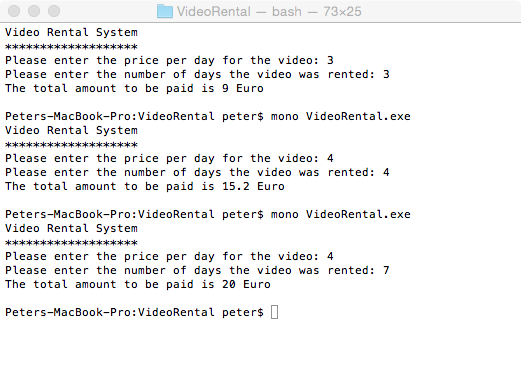
\includegraphics[scale=.7]{SampleOutput.png}
\end{center}

\section{Hinweise}
\begin{enumerate}
	\item Wie im ersten Beispiel zu sehen ist, wird ``normalerweise'' die Verleihgeb�hr durch Multiplikation der Tagesgeb�hr mit der Anzahl der Tage ermittelt. Das gilt aber nur bei einer Verleihdauer von bis zu drei Tagen.
	
	\item Wie im zweiten Beispiel zu sehen ist, wird ab dem vierten Tag die Tagesgeb�hr f�r die restlichen Tage um 20 \% gesenkt, d.h., die Verleihgeb�hr errechnet sich aus $3 \; \textrm{Tage} \cdot 4 \; \textrm{Euro Tagesgeb�hr} + (1 \; \textrm{weiterer Tag} \cdot 4 \cdot 0.8 \; \textrm{um 20 \% reduzierte Tagesgeb�hr}) = 3 \cdot 4 + 3.2 = 15.2$.
	
	\item Wie aus dem dritten Beispiel zu sehen ist, kann der Verleihbetrag 20 Euro nicht �bersteigen.
	
	\item Fehlerhafte Eingaben, wie  Verleihgeb�hren $\leq 0$ und Tagesangaben $< 1$ sollen eine Fehlermeldung ergeben und es soll keine Berechnung erfolgen.\label{hint:wronginput}
	
	\item Das Beispiel ist mit Notepad++ und mit Hilfe des Compileraufrufs in der Eingabeaufforderung zu l�sen.
\end{enumerate}

\section{L�sungsidee}
\begin{enumerate}
	\item Sie pr�fen die Eingaben, ob Sie valide sind (siehe Hinweis~\ref{hint:wronginput}). Wenn diese ok sind, dann kommen folgende Schritte:
	\item Sie legen eine Variable an, die den Gesamtbetrag speichert (beispielsweise {\tt totalAmount}). Welcher Datentyp ist erforderlich?
	\item Wenn die Anzahl der Verleihtage zwischen 1 und 3 ist, berechnen Sie {\tt totalAmount} durch Multiplikation der Tage mit der Tagesgeb�hr.
	\item Sonst:
	\begin{enumerate}
		\item Sie berechnen die Verleihgeb�hren f�r die ersten 3 Tage durch Multiplikation von 3 mit der Tagesgeb�hr.
		\item Sie berechnen die Verleihgeb�hren f�r die restlichen Tage durch Multiplikation der Gesamttage minus 3 mit der reduzierten Tagesgeb�hr (= Tagesgeb�hr $\cdot \; 0.8$).
		\item {\tt totalAmount} ist nun die Summe der beiden oben ermittelten Geb�hren.
	\end{enumerate}
	\item Wenn der Gesamtbetrag $>$ 20 ist, setzen Sie ihn auf 20.
	\item Sie geben das Ergebnis aus.
\end{enumerate}
\section{Source Code Qualit�t}
Achten Sie darauf, dass Sie korrekte Einr�ckungen machen und dass die Variablennamen richtig geschrieben werden (Gro�- und Kleinschreibung).

\end{document}